\chapter{Implementation}
\label{ch:implementation}
This chapter describes the implementation

\note {
\url{https://www.tutorialspoint.com/cassandra/cassandra_introduction.htm}
}


\section{Effects of Replication}
\label{sec:Effects_of_Replication}
\comment{Han siger det er vigtig: \url{https://testdetective.com/performance-testing-vegeta-attack/},}
\comment{3 scale, by RED HAT: \url{https://www.3scale.net/2015/04/how-to-load-test-and-tune-performance-on-your-api-part-i/}}
A benchmarking test of a simple application has been completed to show the impact of replication, and how it improves capacity and thereby level of availability. When developing a microservice architecture it is important to determine the limit for individual service endpoints. Determining whether an application has the proper capacity for the expected load, and how much unexpected load it can handle. Replication of services is one of the main advantages of using microservices. Giving the ability to scale as demand grows and having a healthy level of redundancy if needed. 
Kubernetes was utilized to create a cluster on the Google Cloud Platform (GCP), creating a suitable environment for carrying out the test. Making it possible to change the replication factor after deployment and survey each active node, making usage of Grafana to survey load on individual notes by monitoring CPU and network usage. The application was made available with three different node replication factors: 1,  5 and 10, to investigate the increase of throughput on a single api endpoint. 
The application was load tested with a benchmarking tool running on a separate server in a benchmarking tool developed specifically for the test. By evaluating the responses time and success rate of requests the maximum amount of requests per second for the specific replication factor was determined and evaluated.


\subsubsection{Test Application}
The test application was devloped as a java application, due to the simplicity and good documentation of the available java frameworks, making it possible to develop a test ready application rather confidently. The test application exposes a single API endpoint supporting GET requests, which returns a empty list of simple \textit{Rule} objects, containing a single attribute. The spring boost framework was utilized to create the API endpoint, due to it's simplicity and ease of use. The application was tested locally and containerized using docker, using the spotify \footnote{Docker maven plugin for creating and pushing containerized applications directly with maven \url{https://github.com/spotify/docker-maven-plugin}} docker maven plugin that makes it possible go create and push new docker images to the docker hub\footnote{The image is available on docker hub: \url{https://hub.docker.com/r/ihacheinsen/simple-rest-api/}} using maven. A kubernetes deployment was  used to deploy the application in the cluster, utilizing the Kubernetes functionality to scale the application to the wished amount of replicates for the given test step, delivering good monitoring, making it possible to monitor health and utilization of individual service replicas.

\subsection{Test Tool}
A NodeJS application was developed, to initiate the chosen benchmarking tool and collect results from the test. The application expose a single web page, making it possible to specify the host targeted for load test, number of total requests in each test step, a start rate of requests per second - used to calculate rate at each test step - the start step and a total amounts of steps for the test. 

The application was hosted through GCP on a separate VM instance, located in \textit{europe-west1-c} (a different zone then the cluster hosting the test application) to ensure some 'distance' between the test tool and test application. GCP makes it possible to access created instances through SSH, where the test tool was deployed and monitored using docker.

Load was generated with the benchmarking tool Vegeta\footnote{The Vegeta load testing tool and library can be found on github: \url{https://github.com/tsenart/vegeta}}. Vegeta is a open source library, that makes it possible to generate a high amount of requests directed to any given host, making it possible to tune the test by specifying wished timeout, duration among other parameters, providing several neat commands for generating reports of the test results as well. The test tool initiates Vegeta for each test step, steadily increasing the amount of request per second for each increasing step. Vegeta produce results for each step, which are gathered in a simplified JSON structure for display on the test tool web page. Besides response time, Vegeta gives information about success rate and overall duration of a test, giving more indicators of whether the specific host under test managed to satisfied the load. If a host is overloaded, the duration of the test typically exceeds the predefined duration, due to a high amount of timeouts, giving a poor success rate. Success rate and duration are therefore a product of response time.

\subsection{Test}
The application has been load tested in 20 steps, starting with 100.000 request per second steadily increased by multiplying the start rate with the current step, resulting in a maximum of 200.000 requests per second. Each step sends a total of 100000 requests, resulting in different durations of each test step. The equation for calculating the given duration for a step is seen on figure \ref{fig:implementation_load_duration_equation} below, calculated before initiating each test step.

\begin{figure}[!htb]
  
\includegraphics[width=\textwidth]{implementation_load_duration_equation}  
  \caption{Equation used to calculate duration of each load test step}
  \label{fig:implementation_load_duration_equation}
\end{figure}

This calculation was done to satisfy the parameters of the utilized benchmarking tool Vegeta, that requires a test duration and a amount of requests per second, without the ability to specify a fixed total amount of requests at a given rate.

Each test iteration was done 10 times to account for outliers, creating a reasonable sample basis.


\subsection{Test Results}
The test results are evaluated primarily by judging the response time median at each step for the given cluster configuration. Success rate and duration also contribute to the evaluation, providing useful insights into how successfully the application configuration handled the load. The response time results are visualised in figure \ref{fig:implementation_effect_of_replication_requests}. A response time above 100 ms was deemed unsatisfactory, which was breached for each cluster configuration rather clearly with a enormous spike in response times at a certain load increase. 

\begin{figure}[!htb]
  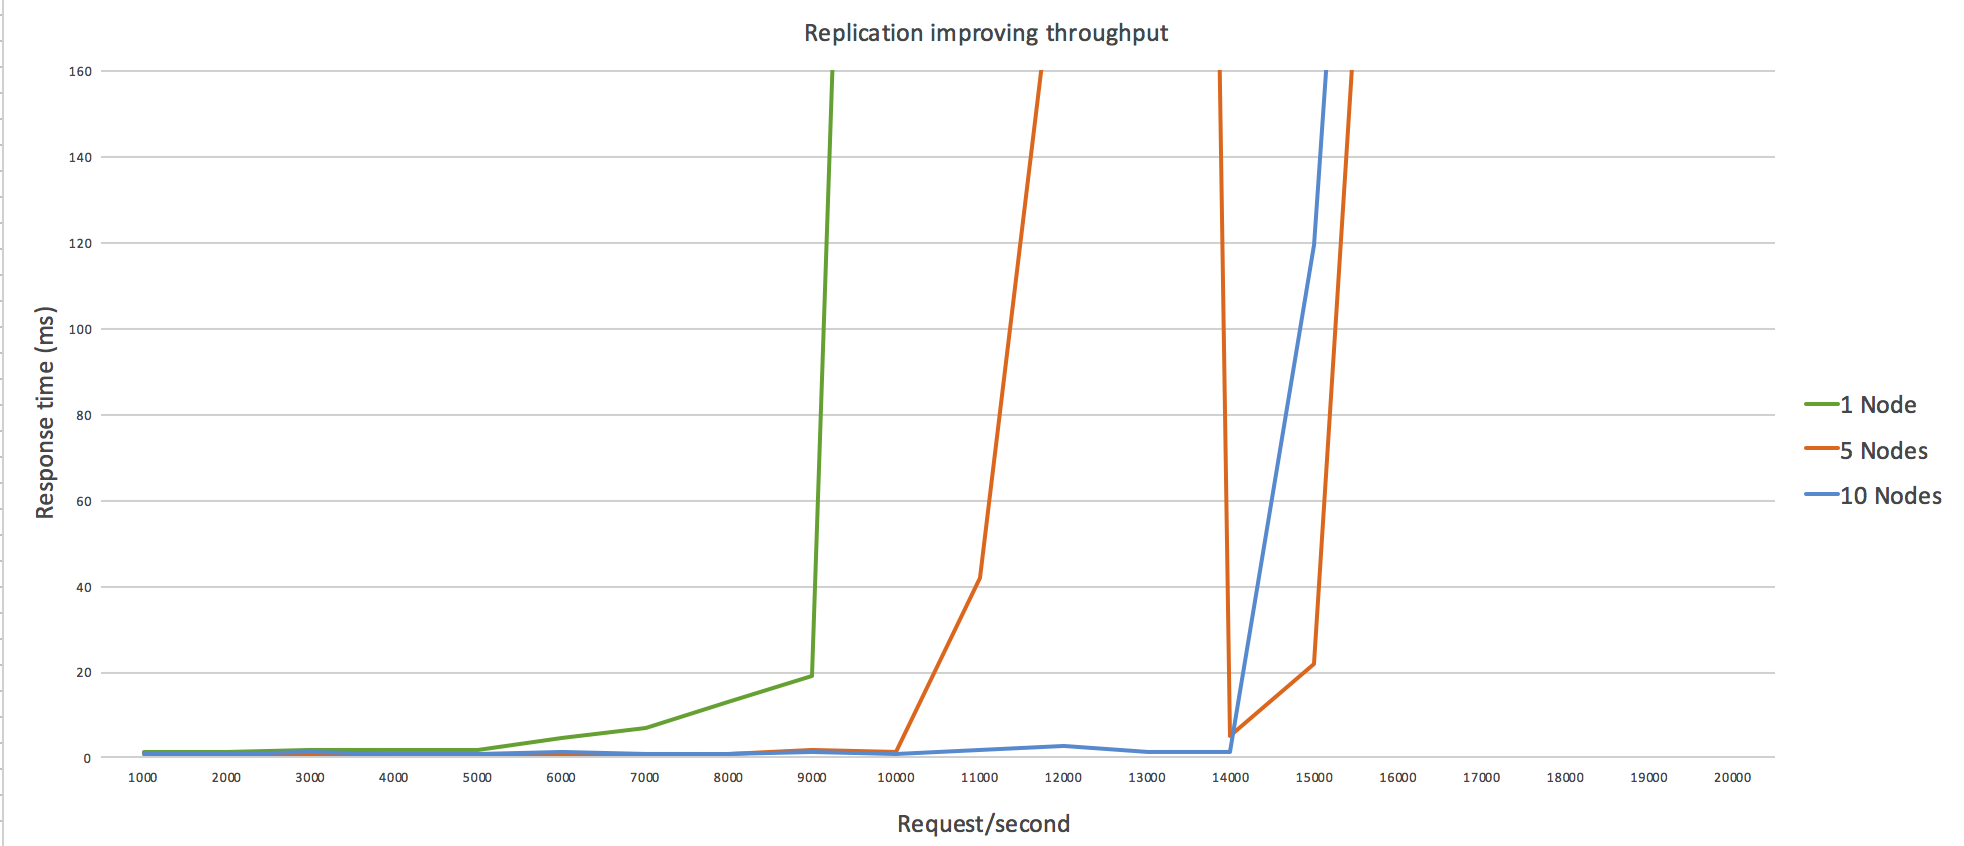
\includegraphics[width=\textwidth]{implementation_effect_of_replication_requests}  
  \caption{Response time for each cluster configuration}
  \label{fig:implementation_effect_of_replication_requests}
\end{figure}

Test results are gathered for each configuration, creating an average across all 10 tests executed for each cluster configuration. The results clearly show a improvement in maximum throughput for the application, with the lowest attainable throughput at 1 node, and a highest at 10 nodes. The results show how replication factor of the test application is a determining factor for maximum throughput, creating clear boundaries for when a application is able to satisfy a given load. The application was able to satisfy the following loads at different replication factors:

\begin{center}
\begin{tabular}{ |p{2cm}|p{5cm}|  }
 \hline
{\textbf{Nodes}} & {\textbf{Requests per Second}}\\
 \hline
 \textbf{1} & 9000 r/s\\
 \hline
 \textbf{5} & 11000 r/s\\ 
 \hline
 \textbf{10} & 14000 r/s\\ 
 \hline
\end{tabular}
\end{center}

Measurements after reaching a configurations seemingly maximum throughput gives very mixed results, and should not be regarded. The figure clearly shows how the 5 node cluster configuration delivers bad response times between 10.000 and 14.000 requests per second, while reappearing in the graph after 14.000 request per second. It would seem that the cluster configuration is able to recover from a constant flow of requests, for a short period of time, in the end the configuration does not manage to uphold the required response time at the high load.

The CPU load for nodes in the different cluster configurations was exported from the default Kubernetes cluster monitoring tool Grafana, visualised below in figure \ref{fig:implementation_effect_of_replication_cpu}. It is clearly visible on the graph that nodes in the 1 node cluster configuration is drastically more loaded, whereas nodes in 5 and 10 node configurations are less loaded across test runs.

\begin{figure}[!htb]
  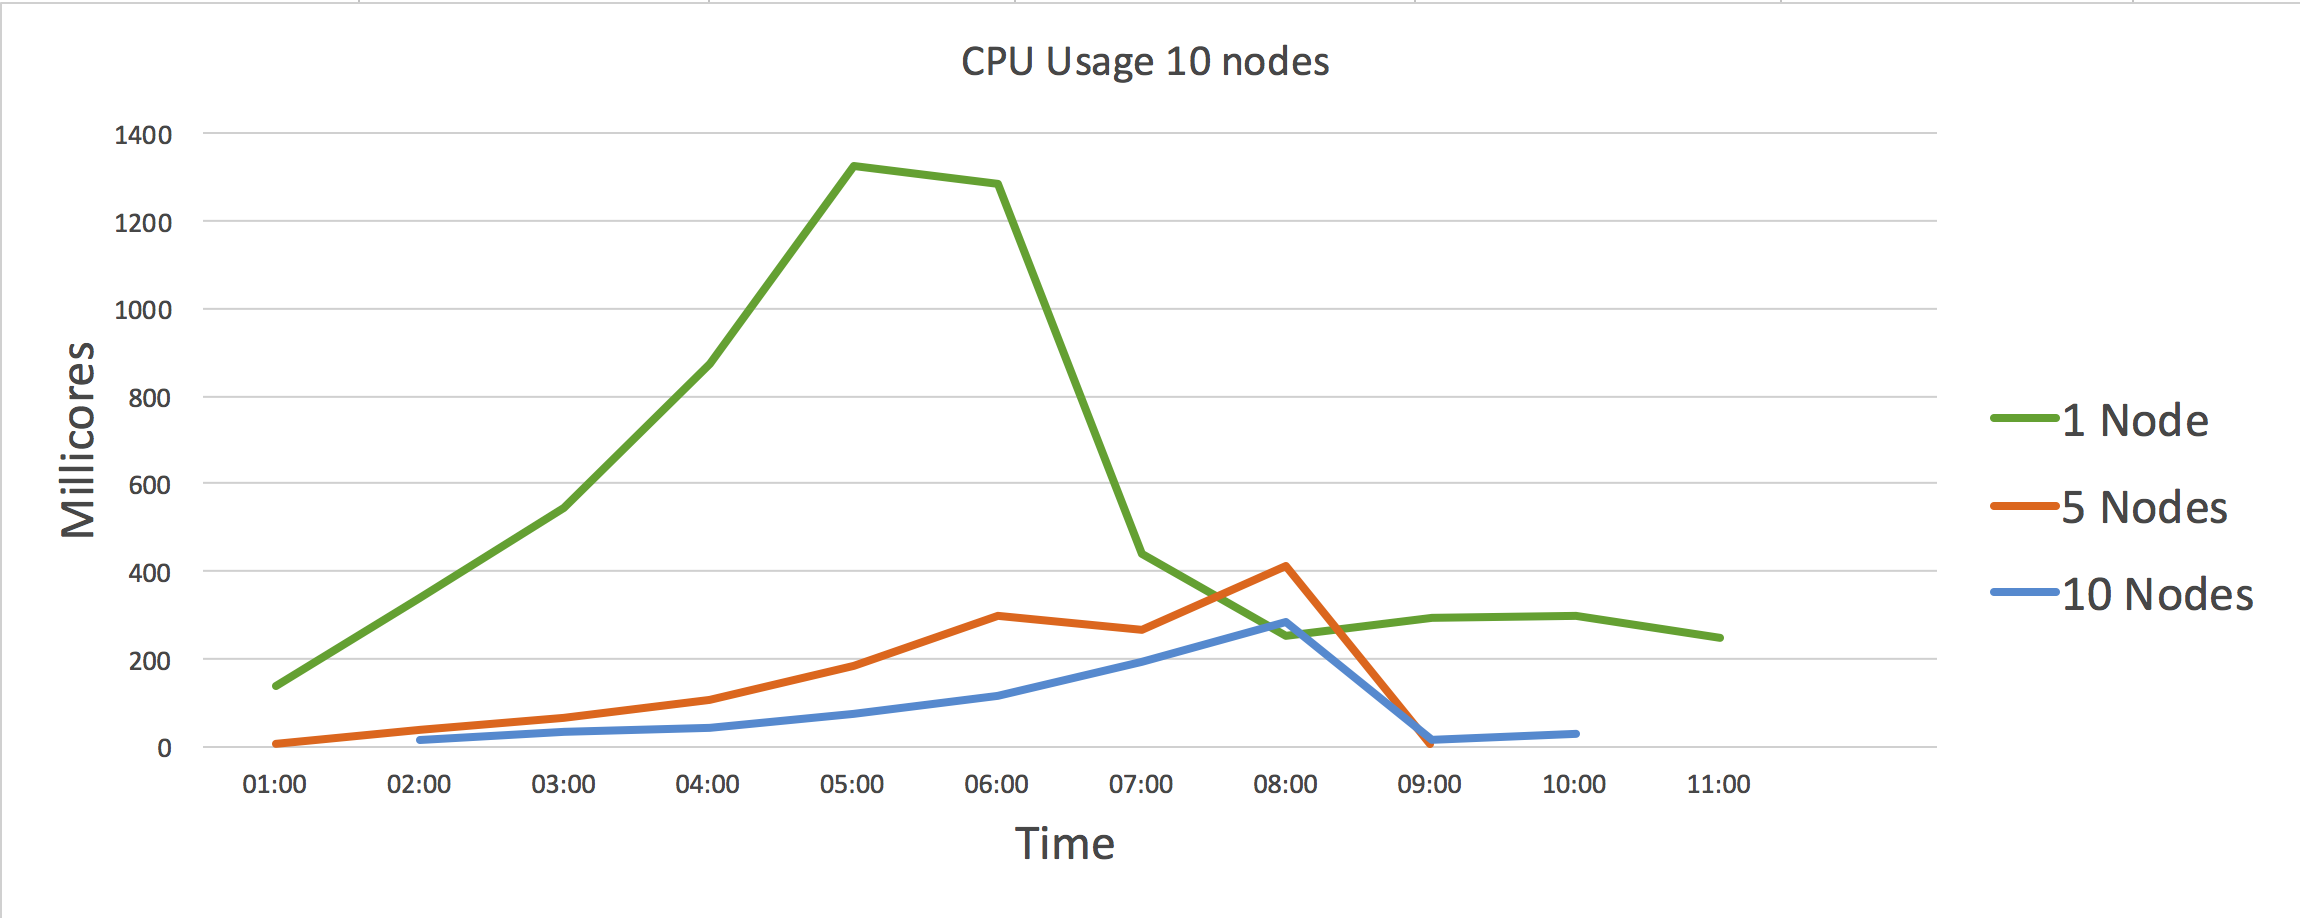
\includegraphics[width=\textwidth]{implementation_effect_of_replication_cpu}  
  \caption{CPU usage on individual nodes, in different cluster configurations}
  \label{fig:implementation_effect_of_replication_cpu}
\end{figure}

It has to be noted that several factors are contributing to the discrepancy between the different CPU datasets. The CPU data has a low sampling rate - the default sampling rate for CPU and network monitoring is 1 minute -, and data was manually exported, making the collection sub optimal. As mentioned earlier, fail-overs of cluster configurations, due to reaching maximum throughput, extends the overall duration, creating variations in test runs duration. The exported data is therefore fitted, giving the most accurate representation.

\subsubsection{Limiting Factors}
Many factors was found to affect the test results, which are important to consider when doing load testing.The test tool was hosted on a separate machine to minimize external factors and create 'distance' to the application under test: Several provisioning sizes were tried before choosing a VM instance with 8 CPU's, as this was the smallest machine capable of delivering the required maximum load of 20.000 requests per second. Choosing smaller VM instances decreased the reliability of the test tool due to exhaustion of the available processor power.

Several testing tools were tried and tested, Vegeta made it possible to emit the required amount of requests simultaneously, other tools did not deliver in the same way for this test. Reflecting about which tool serves the purpose of the specific test best is advised. The different available open source tools are designed with different purposes in mind, having a tool not meeting expectations is a potent source for error, hiding in the test tool and therefore not the test application.


The test tool makes it easy to initiate new test iterations, and gathers results for further review. Having a impression of the capacity for a given application makes it possible to quantify whether application services live up to the requirements, and not as the systems new bottleneck. Identifying the correct minimum and maximum load, as well as identifying expected performance can be a tedious task, immediate by the test tool, making it easy to try out different configurations. Hosting the test application in a cluster, where limiting factors can be determined and changed by configuration makes it possible to evaluate the test application in different setups, identifying the optimal configuration.



\section{Circuit breaker}


\note {

\subsection{Distributed databases}

}

\note {
Notes for:
"GOTO 2012 • Introduction to NoSQL • Martin Fowler" \url{https://www.youtube.com/watch?v=qI_g07C_Q5I}:

Column family:\\
You want to store things that are retreived together should be stored together. 

If are gonna distribute data, what you wanna do is you wanna distribute data that tends to be accessed together

Aggregate tells you what data can be accessed together. Different aggregates on different nodes in the cluster. Aggregate orientation naturally fits very nicely with storing data on clusters.


Changing aggregate structure is very costly. Usually hash maps is used

Aggregate is an advantage if data is pushed back and forth using the same aggregate. Otherwise it is vary ineffective.

Two types of databases:\\
Aggregate-oriented:\\
Document
Column.family
Key-value

ACID:\\
Graph
\\

Consistency is twofold:
\textbf{Logical}


\textbf{Replication}



Distributing data, broadly you can talk about it in two ways:
\textbf{Sharding}: data only lives in one place, spread out on several machines
\textbf{Replicate data}: Same data in a lot of places. 
Advantages for performance, several machines can handle same pool of requests.
Resilience, if one node goes down, others have the same data and can handle requests.
New class of consistency problems come in:

Choice between consistency and availability.\\
Consistency - my service is not always available, but always consistent.\\
Availability- my service is always available, but might introduce inconsistency.\\
It is always a domain/business choice, what is more important, availability or consistency.

CAP theorem: - As soon as you have a distributed system
If you get a network partition, do you want to be available, or consistent.
It is a spectrum, it can vary between transactions.

most of the time you are not trading of availability for consistency, not even network partitioning.\\
A lot of the time it is consistency vs. response time, nodes needs to communicate, which takes times.\\
more broadly it is safely and liveness.<- look into this? \\

Have to think about consistency issues differently, essentially because you have a different data model and the possibility of replicated data. In particular you have to think about the availability consistency tradeoff, and the decisions should be based on domain/business.\\

Too drivers towards noSQL:
\textbf{Large amount of data}
If you have more data, than fits on one server. Running relational database across clusters, is not good.\\
There is tons of data coming, large scale data problem is only gonna grow. 

\textbf{Easier development} - Most common reason why people change to noSQL right now (2012)
Most people are actually not interested in big data.
Most wants easier development, many works with aggregates of data, the 'impedance mismatch problem' can be reduced. Relational database model does not necessarily fit the domain.

\textbf{Other drivers:}
Integration issues goes away, because integration database is not a good thing. This gives a lot of freedom to choose new databases.

Data warehouse projects, a lot of stakeholders, a lot of different data from different subsystems. noSQL databases can help in different ways, not all are equally good to solve these problems, but graph especially is very good.

\textbf{Future brings:}
Polyglot persistence. Many different databases, SQL still play a big role.Different natures of problems, different databases.

A lot of problems. Which database is the best for this problem. 

Tools and knowledge is not good enough for noSQL yet. Consistency issues can still cause a lot of problems.

Rapid time to market, easy development is very important. Data intensity is very high. Is you project really important, strategic important, "Strategic project", it is worth taking on the extra risks the unknowns of dealing with immature technology. Utility project: Not vital to the business, choose a familiar for a few years.

}

